\documentclass{article}

\providecommand{\finishEntry}[1][]{\end{document}} % please don't change this line
\providecommand{\startEntry}[1][]{\begin{document}} % please don't change this line


\usepackage[english]{babel}
\usepackage{amsmath}
\usepackage{amssymb}
\usepackage{amsthm}
\usepackage{physics} % for \abs{}
\usepackage{bm} % for \bm bold text

\usepackage{graphicx}

\graphicspath{ {./figures/} }

\DeclareMathOperator{\im}{Im} %Image

\newcommand{\nat}{\mathbb{N}}
\newcommand{\re}{\mathbb{R}}
\newcommand{\rat}{\mathbb{Q}} %rationals

\newcommand{\transpose}{\intercal}  %why on earth is this thing called an `intercal'?
\newcommand{\del}{\partial}

\newcommand{\dx}[1][x]{\text{d} #1 }  %usage $\dx$ -> dx, or $\dx[V]$ -> dV

\newcommand{\floor}[1]{\lfloor #1 \rfloor}
\newcommand{\ceil}[1]{\lceil #1 \rceil}

\theoremstyle{plain}
\newtheorem{thm}{Theorem}[section]
\newtheorem{lem}[thm]{Lemma}
\newtheorem{prop}[thm]{Proposition}
\newtheorem*{thmno}{Theorem}
\newtheorem*{lemno}{Lemma}
\newtheorem*{propno}{Proposition}


\theoremstyle{definition}
\newtheorem{defn}{Definition}[section]
\newtheorem*{defno}{Definition}

\theoremstyle{remark}
\newtheorem{rem}{Remark}
\newtheorem*{remno}{Remark}

% Please edit this file as you please so that it does what you want it to. ()
% This file is intended to contain all of the course independent macros and packages.
% If you need a specific package or command for just one course, that should be defined in that course's "preamble.tex"

\renewcommand{\startEntry}[1][]{} % this line must stay here to ensure the program works
\renewcommand{\finishEntry}[1][]{} % this line must stay here to ensure the program works
\graphicspath{ {D:/All other files/Lect_Stack/Example Usecase/Courses/Optimisation/figures/} }
\def\DONOTUSERELATIVEPATHS{0}
\documentclass{article}

\providecommand{\finishEntry}[1][]{\end{document}} % please don't change this line
\providecommand{\startEntry}[1][]{\begin{document}} % please don't change this line


\usepackage[english]{babel}
\usepackage{amsmath}
\usepackage{amssymb}
\usepackage{amsthm}
\usepackage{physics} % for \abs{}
\usepackage{bm} % for \bm bold text

\usepackage{graphicx}

\graphicspath{ {./figures/} }

\DeclareMathOperator{\im}{Im} %Image

\newcommand{\nat}{\mathbb{N}}
\newcommand{\re}{\mathbb{R}}
\newcommand{\rat}{\mathbb{Q}} %rationals

\newcommand{\transpose}{\intercal}  %why on earth is this thing called an `intercal'?
\newcommand{\del}{\partial}

\newcommand{\dx}[1][x]{\text{d} #1 }  %usage $\dx$ -> dx, or $\dx[V]$ -> dV

\newcommand{\floor}[1]{\lfloor #1 \rfloor}
\newcommand{\ceil}[1]{\lceil #1 \rceil}

\theoremstyle{plain}
\newtheorem{thm}{Theorem}[section]
\newtheorem{lem}[thm]{Lemma}
\newtheorem{prop}[thm]{Proposition}
\newtheorem*{thmno}{Theorem}
\newtheorem*{lemno}{Lemma}
\newtheorem*{propno}{Proposition}


\theoremstyle{definition}
\newtheorem{defn}{Definition}[section]
\newtheorem*{defno}{Definition}

\theoremstyle{remark}
\newtheorem{rem}{Remark}
\newtheorem*{remno}{Remark}

% Please edit this file as you please so that it does what you want it to. ()
% This file is intended to contain all of the course independent macros and packages.
% If you need a specific package or command for just one course, that should be defined in that course's "preamble.tex"

% a friendly reminder to use \startEntry and \endEntry instead of \begin{document} and \end{document}
% Lect_Stack will replace all of the ##<identifier>## strings with the text that they represent
% If there are and ##<identifier>## strings left when you try to latexmk this file we make no guarantees that this will compile correctly. (Although it probably will still do something sensible)

\begin{document}
\author{Henry}
\title{Optimisation.tex}
\maketitle
\tableofcontents

\documentclass{article}

\providecommand{\finishEntry}[1][]{\end{document}} % please don't change this line
\providecommand{\startEntry}[1][]{\begin{document}} % please don't change this line


\usepackage[english]{babel}
\usepackage{amsmath}
\usepackage{amssymb}
\usepackage{amsthm}
\usepackage{physics} % for \abs{}
\usepackage{bm} % for \bm bold text

\usepackage{graphicx}

\graphicspath{ {./figures/} }

\DeclareMathOperator{\im}{Im} %Image

\newcommand{\nat}{\mathbb{N}}
\newcommand{\re}{\mathbb{R}}
\newcommand{\rat}{\mathbb{Q}} %rationals

\newcommand{\transpose}{\intercal}  %why on earth is this thing called an `intercal'?
\newcommand{\del}{\partial}

\newcommand{\dx}[1][x]{\text{d} #1 }  %usage $\dx$ -> dx, or $\dx[V]$ -> dV

\newcommand{\floor}[1]{\lfloor #1 \rfloor}
\newcommand{\ceil}[1]{\lceil #1 \rceil}

\theoremstyle{plain}
\newtheorem{thm}{Theorem}[section]
\newtheorem{lem}[thm]{Lemma}
\newtheorem{prop}[thm]{Proposition}
\newtheorem*{thmno}{Theorem}
\newtheorem*{lemno}{Lemma}
\newtheorem*{propno}{Proposition}


\theoremstyle{definition}
\newtheorem{defn}{Definition}[section]
\newtheorem*{defno}{Definition}

\theoremstyle{remark}
\newtheorem{rem}{Remark}
\newtheorem*{remno}{Remark}

% Please edit this file as you please so that it does what you want it to. ()
% This file is intended to contain all of the course independent macros and packages.
% If you need a specific package or command for just one course, that should be defined in that course's "preamble.tex"

% a friendly reminder to use \startEntry and \endEntry instead of \begin{document} and \end{document}
\startEntry{}
Today's lecture will be about frying.
\section{How to fry and egg}
There are lots of different ways to fry an egg, but they all do a similary thing: Heat the egg up so that it cooks in, but in a frying pan. I will now describe how to do this.
\begin{enumerate}
\item Put pan on heat
\item Add fat (oil, butter)
\item Let oil heat up a bit
\item Add egg
\item (Optional) Stir egg violently
\item When egg is no longer liquid, it is cookes
\item Remove egg
\item Take pan off heat
\end{enumerate}
I should probably mention that I have never cooked an egg before.
This is what it shoud look like:
\begin{figure}[h]
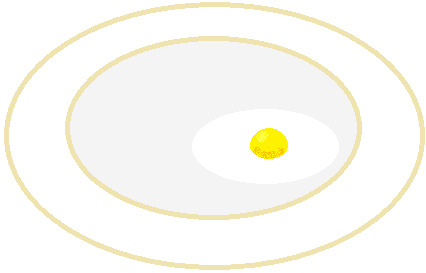
\includegraphics[width=8cm]{Egg_on_plate.png}
\end{figure}


Now isn't that a nice egg?
\finishEntry{}
\documentclass{article}

\providecommand{\finishEntry}[1][]{\end{document}} % please don't change this line
\providecommand{\startEntry}[1][]{\begin{document}} % please don't change this line


\usepackage[english]{babel}
\usepackage{amsmath}
\usepackage{amssymb}
\usepackage{amsthm}
\usepackage{physics} % for \abs{}
\usepackage{bm} % for \bm bold text

\usepackage{graphicx}

\graphicspath{ {./figures/} }

\DeclareMathOperator{\im}{Im} %Image

\newcommand{\nat}{\mathbb{N}}
\newcommand{\re}{\mathbb{R}}
\newcommand{\rat}{\mathbb{Q}} %rationals

\newcommand{\transpose}{\intercal}  %why on earth is this thing called an `intercal'?
\newcommand{\del}{\partial}

\newcommand{\dx}[1][x]{\text{d} #1 }  %usage $\dx$ -> dx, or $\dx[V]$ -> dV

\newcommand{\floor}[1]{\lfloor #1 \rfloor}
\newcommand{\ceil}[1]{\lceil #1 \rceil}

\theoremstyle{plain}
\newtheorem{thm}{Theorem}[section]
\newtheorem{lem}[thm]{Lemma}
\newtheorem{prop}[thm]{Proposition}
\newtheorem*{thmno}{Theorem}
\newtheorem*{lemno}{Lemma}
\newtheorem*{propno}{Proposition}


\theoremstyle{definition}
\newtheorem{defn}{Definition}[section]
\newtheorem*{defno}{Definition}

\theoremstyle{remark}
\newtheorem{rem}{Remark}
\newtheorem*{remno}{Remark}

% Please edit this file as you please so that it does what you want it to. ()
% This file is intended to contain all of the course independent macros and packages.
% If you need a specific package or command for just one course, that should be defined in that course's "preamble.tex"

% a friendly reminder to use \startEntry and \endEntry instead of \begin{document} and \end{document}
\startEntry{}
\section{Best Egg Cooking stratergy}
We want to cook the egg in the best way, but what should "best" mean here? Clearly the quality of the final egg should matter, but to make the question more interesting we will consider one other factor, the enjoyment of cooking the egg in the first place. You enjoy cooking an egg more if it looks and smells tastier, so the total enjoyment you get is an integral of the following form \[ \text{Enjoyment} = \int_{t_\text{start}}^{t_\text{end}} \text{tastiness}(t) \,\dx[t]\]
We can draw a diagram for this, because why not:
\begin{figure}[h]
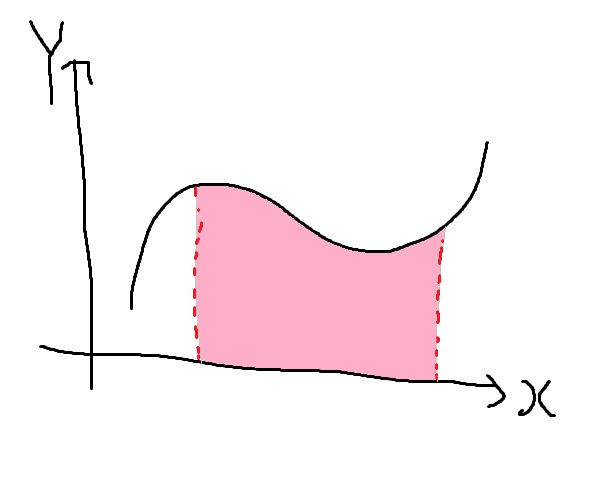
\includegraphics[width = 6cm]{area_under_graph.jpg}
\end{figure}


Our final total goodness function becomes:
\[ \text{Goodness}(T) = \int_{t_\text{start}}^{T} \text{tastiness}(t) \,\dx[t] + \text{tastiness}(T) \]
We will finish this off next time.
\finishEntry{}
\documentclass{article}

\providecommand{\finishEntry}[1][]{\end{document}} % please don't change this line
\providecommand{\startEntry}[1][]{\begin{document}} % please don't change this line


\usepackage[english]{babel}
\usepackage{amsmath}
\usepackage{amssymb}
\usepackage{amsthm}
\usepackage{physics} % for \abs{}
\usepackage{bm} % for \bm bold text

\usepackage{graphicx}

\graphicspath{ {./figures/} }

\DeclareMathOperator{\im}{Im} %Image

\newcommand{\nat}{\mathbb{N}}
\newcommand{\re}{\mathbb{R}}
\newcommand{\rat}{\mathbb{Q}} %rationals

\newcommand{\transpose}{\intercal}  %why on earth is this thing called an `intercal'?
\newcommand{\del}{\partial}

\newcommand{\dx}[1][x]{\text{d} #1 }  %usage $\dx$ -> dx, or $\dx[V]$ -> dV

\newcommand{\floor}[1]{\lfloor #1 \rfloor}
\newcommand{\ceil}[1]{\lceil #1 \rceil}

\theoremstyle{plain}
\newtheorem{thm}{Theorem}[section]
\newtheorem{lem}[thm]{Lemma}
\newtheorem{prop}[thm]{Proposition}
\newtheorem*{thmno}{Theorem}
\newtheorem*{lemno}{Lemma}
\newtheorem*{propno}{Proposition}


\theoremstyle{definition}
\newtheorem{defn}{Definition}[section]
\newtheorem*{defno}{Definition}

\theoremstyle{remark}
\newtheorem{rem}{Remark}
\newtheorem*{remno}{Remark}

% Please edit this file as you please so that it does what you want it to. ()
% This file is intended to contain all of the course independent macros and packages.
% If you need a specific package or command for just one course, that should be defined in that course's "preamble.tex"

% a friendly reminder to use \startEntry and \endEntry instead of \begin{document} and \end{document}
\startEntry{}
\subsection{Finalae}
To find the perfect time for peak overall goodness, you should refer to Part IB Optimisation and apply the methods there to this problem.
\finishEntry{}
\input preamble.tex

\startEntry{}
\section{Mathematical eggs}
How many eggs should you eat? Who knows. All I know is that I want an excuse to have some more images and formulae and things.
Let's draw a fuction.
\section{The Egg equation}
The quality of a cooked egg varies with the time taken to cook it. X is in minutes and Y is tastiness. A good approximation for this is \[x^3 - 6x^2 + 11x - 4\] for $x \in [1/2, 5/2]$.
This function looks a bit like this in the region we want to consider:
\begin{figure}[h]
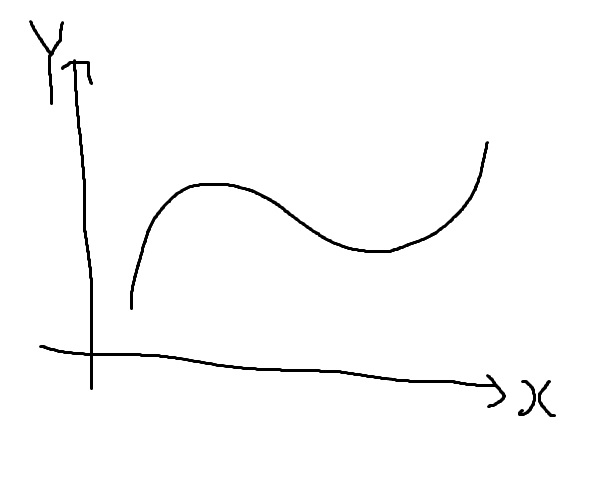
\includegraphics[height = 7cm]{simple_graph.jpg}
\end{figure}

Next time we will analyse this function and try to find a good way to cook the egg.
\finishEntry{}
\documentclass{article}

\providecommand{\finishEntry}[1][]{\end{document}} % please don't change this line
\providecommand{\startEntry}[1][]{\begin{document}} % please don't change this line


\usepackage[english]{babel}
\usepackage{amsmath}
\usepackage{amssymb}
\usepackage{amsthm}
\usepackage{physics} % for \abs{}
\usepackage{bm} % for \bm bold text

\usepackage{graphicx}

\graphicspath{ {./figures/} }

\DeclareMathOperator{\im}{Im} %Image

\newcommand{\nat}{\mathbb{N}}
\newcommand{\re}{\mathbb{R}}
\newcommand{\rat}{\mathbb{Q}} %rationals

\newcommand{\transpose}{\intercal}  %why on earth is this thing called an `intercal'?
\newcommand{\del}{\partial}

\newcommand{\dx}[1][x]{\text{d} #1 }  %usage $\dx$ -> dx, or $\dx[V]$ -> dV

\newcommand{\floor}[1]{\lfloor #1 \rfloor}
\newcommand{\ceil}[1]{\lceil #1 \rceil}

\theoremstyle{plain}
\newtheorem{thm}{Theorem}[section]
\newtheorem{lem}[thm]{Lemma}
\newtheorem{prop}[thm]{Proposition}
\newtheorem*{thmno}{Theorem}
\newtheorem*{lemno}{Lemma}
\newtheorem*{propno}{Proposition}


\theoremstyle{definition}
\newtheorem{defn}{Definition}[section]
\newtheorem*{defno}{Definition}

\theoremstyle{remark}
\newtheorem{rem}{Remark}
\newtheorem*{remno}{Remark}

% Please edit this file as you please so that it does what you want it to. ()
% This file is intended to contain all of the course independent macros and packages.
% If you need a specific package or command for just one course, that should be defined in that course's "preamble.tex"

% a friendly reminder to use \startEntry and \endEntry instead of \begin{document} and \end{document}
\startEntry{}
Hi here is some example text

\section{How to boil and egg}
You need to do a few things to boil an egg:
\begin{enumerate}
\item Get an egg
\item Heat up water to boiling
\item Place the egg gently in the boiling water for the right amount of time
\item Remove egg
\end{enumerate}
So in conclusion, you should probably google how to boil an egg rather than following these instructions.
\finishEntry{}



\end{document}